\section{Afgeleiden}

\subsection{Inleidend voorbeeld}
\begin{minipage}{.25\linewidth}
	\raggedright
	
\includegraphics[width=4cm]{6_afgeleiden_integralen/inputs/QR_Code_INLEIDENDVB_module6new}
\end{minipage}
\begin{minipage}{.7\linewidth}
	Zie filmpje MOOC.
\end{minipage}

\subsection{Algemeenheden}

\emph{Algemeenheden}

In de algemene definities is $f(x)$ het voorschrift van een functie $f$ en $a \in \dom (f)$ zodat $f$ continu is op een omgeving van $a$.
Intu\"itief betekent dit dat een open interval $I \subset \dom (f)$ bestaat dat $a$ bevat en zodat de grafiek van $f$ boven het interval $I$ geen ''sprongen'' vertoont.\vspace{5mm}

\begin{voorbeeld}
	In het inleidende voorbeeld is $f(x)=1,5+50 x -4,9 x^2$, $\dom (f)= \mathbb{R}$ en $a=2$.
	Deze functie is continu in 2. Je ziet hieronder de grafiek van de functie.
	\begin{figure}[h]
		\begin{center}
			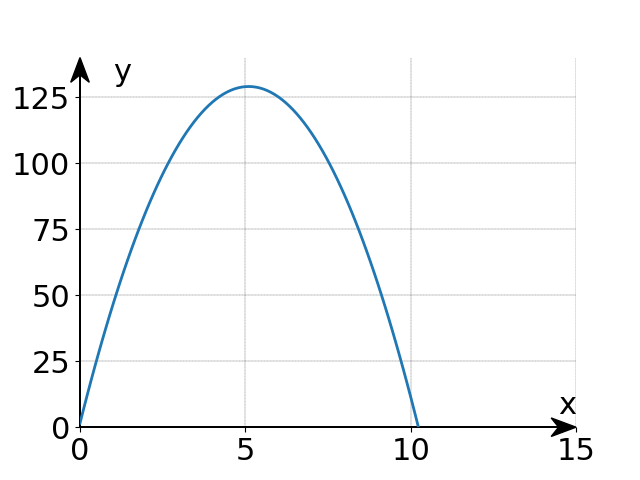
\includegraphics[height=5 cm]{6_afgeleiden_integralen/inputs/1_2_vb1}
		\end{center}
	\end{figure}
\end{voorbeeld}

Naar analogie met dit inleidende voorbeeld introduceren we de volgende definitie.

\begin{definitie}
	Als de limietwaarde van $\frac{f(a+\Delta x)-f(a)}{\Delta x}$ voor $\Delta x = 0$ een re\"eel getal is dan heet dat re\"eel getal de. afgeleide van $f$ in $a$.
	In dat geval zeg je dat $f$ afleidbaar is in $a$
\end{definitie}


\begin{notatie}
	Als $y=f(x)$ afleidbaar is in $a$ dan zijn volgende notaties toegelaten om de afgeleide van $f$ in $a$ aan te duiden
	\[f'(a), Df(a), \frac{d}{dx}f(a)\]
\end{notatie}


\begin{voorbeeld}
	In het inleidend voorbeeld heb je voor de functie  $f(x)=1,5+50 x -4,9 x^2$ gevonden dat deze afleidbaar is in 2 en voor de afgeleide in 2 heb je gevonden dat $Df(2)=30,4$.
\end{voorbeeld}\vspace{0,5 cm}

Vanuit het inleidende voorbeeld ken je een betekenis voor de afgeleide van een functie $f$ in $a$.\vspace{0,2 cm}

\fbox{
	\begin{minipage}{\textwidth}
		De afgeleide van $f$ in $a$ is de snelheid waarmee de functiewaarde $f(x)$ verandert als $x$ verandert vertrekkende met de waarde $x=a$
\end{minipage}}\vspace{0,5 cm}

De afgeleide heeft ook een belangrijke meetkundige betekenis.\vspace{0,2 cm}

\fbox{
	\begin{minipage}{\textwidth}
		De afgeleide van $f$ in $a$ is de richtingsco\"effici\"ent van de raaklijn aan de grafiek van $f$ in het punt $P(a,f(a))$.
\end{minipage}}\vspace{0,2 cm}

De verklaring hiervan zie je in de animatie in de MOOC.

\begin{minipage}{.25\linewidth}
	\raggedright
	
\includegraphics[width=4cm]{6_afgeleiden_integralen/inputs/QR_Code_AFGANIMATIE_module6_1new}
\end{minipage}
\begin{minipage}{.7\linewidth}
	Zie filmpje MOOC.
\end{minipage}

\begin{voorbeeld}
	Voor de functie $f(x)=1,5+50 x -4,9 x^2$ uit het inleidend voorbeeld berekende je dat $Df(2)=30,4$.
	Het punt op de grafiek bij $x=2$ is het punt met co\"ordinaten $P(2;81,9)$.
	De vergelijking van de raaklijn aan de grafiek van $f$ in $P$ is
	\[
	y-81,9=30,4(x-2)
	\]
	of nog
	\[
	y=30,4x+21,1
	\]
	
	\begin{figure}[h]
		\begin{center}
			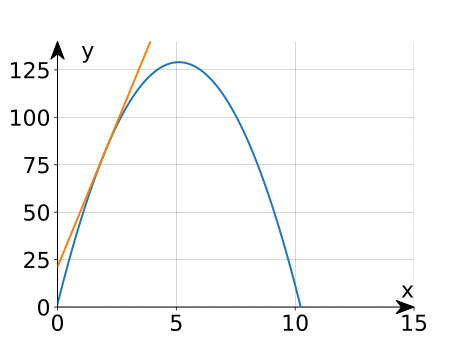
\includegraphics[height=5 cm]{6_afgeleiden_integralen/inputs/1_2_vb3}
		\end{center}
	\end{figure}
\end{voorbeeld}\vspace{0,5 cm}

\begin{definitie}
	Als je $a$ laat vari\"eren in de punten waarin een functie $f$ afleidbaar is dan verandert $Df(a)$ (meestal) ook.
	Je bekomt dan de afgeleide functie van $f$.
\end{definitie}

\begin{notatie}
Voor het aanduiden van de afgeleide functie van een functie $y=f(x)$ mag je de volgende notaties gebruiken
\[f',Df,\frac{df}{dx}\]
\end{notatie}

\subsection{Afgeleide raaklijn}

\begin{minipage}{.25\linewidth}
	\raggedright
	
\includegraphics[width=4cm]{6_afgeleiden_integralen/inputs/QR_Code_AFGRAAKLIJN_module6new}
\end{minipage}
\begin{minipage}{.7\linewidth}
	Zie filmpje MOOC.
\end{minipage}

\subsection{Afgeleiden van veeltermfuncties}

\subsubsection{Afgeleide van een constante functie}

Voor $c\in \mathbb{R}$ is $y=c$ het voorschrift van een constante functie.
Intu\"itief (afgeleide geeft snelheid aan waarmee een functiewaarde verandert) is $D(c)=0$.\vspace{3 mm}

Via de definitie:

\begin{equation*}
f(a)=c \text{ en } f(a+\Delta x)= c \text{ dus } \frac{y(a+ \Delta x)-y(a)}{\Delta x}=\frac {c-c}{\Delta x}=0
\end{equation*}

In de limiet als $\Delta x$ nul wordt blijft dit 0.
Je bekomt 
\[D(c)=0\]

\subsubsection{Afgeleide van de identieke functie}

Het voorschrift $f(x)=x$ is het voorschrift van de identieke functie.
Waaraan is $D(x)$ gelijk?\vspace{3mm}

Via de definitie:

\begin{equation*}
f(a)=a \text{ en } f(a+\Delta x)=a+\Delta x \text{ dus }\frac{y(a+\Delta x)-y(a)}{\Delta x}=\frac{a+\Delta x -a}{\Delta x}=1
\end{equation*}

In de limiet als als $\Delta x$ nul wordt blijft dit 1.
Je bekomt 
\[D(x)=1\]

\subsubsection{Afgeleide van $y=x^2$}

Voor $f(x)=x^2$ is

\begin{eqnarray*}
f(a)=a^2 \text{ en } f(a+\Delta x)=(a+\Delta x)^2=a^2+2a\Delta x + \Delta x^2 \\
\text{dus }
\frac{y(a+\Delta x)-y(a)}{\Delta x}=\frac{2a \Delta x +\Delta x^2}{\Delta x}=2a+ \Delta x.
\end{eqnarray*}

In de limiet als $\Delta x$ nul wordt dan bekom je $2a$.
Je bekomt $Dy(a)=2a$ en daarom 
\[D(x^2)=2x\]

\subsubsection{Afgeleide van $y=x^n$}

Algemeen geldt voor $n\in \mathbb{N}$ dat 
\[D(x^n)=nx^{n-1}\]

Merk op, als $n=0$ dan geeft dit $D(x^0)=0x^{-1}=0$.
Omdat $x^0=1$ geeft dit $D(1)=0$.
Dat komt overeen met de afgeleide van een constante functie.

\subsubsection{Afgeleiden van veeltermfuncties}

Uit de afgeleide van $y=x^n$ met $n\in \mathbb{N}$ volgt dat je door middel van de volgende twee rekenregels van alle veeltermfuncties de afgeleide kunt berekenen.

\begin{eigenschap} Afgeleide van een som : \\
\[ D(f+g)=Df+Dg\]
\end{eigenschap}

\begin{eigenschap} Afgeleide van een functie vermenigvuldigd met een constante :
\[ D(cf)=cD(f)\]
\end{eigenschap}

\begin{voorbeeld}
	\begin{equation*}
	\begin{split}
	D(5x^3-&7x^2+18x-9)\\
	&=D(5x^3)+D(-7x^2)+D(18x)+D(9) \text{ (rekenregel som)}\\
	&=5D(x^3)-7D(x^2)+18D(x)+D(9) \text{ (rekenregel product met c)}\\
	&=5.3x^2-7.2x+18.1+0 \text{ $(D(x^n)=nx^{n-1})$}\\
	&=15x^2-14x+18
	\end{split}
	\end{equation*}
\end{voorbeeld}

\begin{voorbeeld}
	Bekijk terug de functie uit het beginvoorbeeld
	\[
	f(x)=1,5+50t-4,9t^2
	\]
	Met de rekenregels en afleiden van $x^n$ bekom je
	\[
	Df(x)=50-9,8t
	\]
	Merk op dat je door invullen vindt $Df(2)=50-9,8.2=30,4$.
	Dit is het resultaat dat we eerder gevonden hadden.
\end{voorbeeld}

Uit de twee rekenregels volgt ook
\begin{eigenschap} Algeleide van een verschil
	
\[D(f-g)=Df-Dg\]
\end{eigenschap}\vspace{5 mm}
\begin{eigenschap}
	De afgeleide $D(x^n)=nx^{n-1}$ geldt algemener voor alle $n\in \mathbb{R}$.
\end{eigenschap}

\begin{voorbeeld}
	$D(\sqrt[5]{x})=D(x^{1/5})=\frac{1}{5}x^{-4/5}=\frac{1}{5x^{4/5}}=\frac{1}{5\sqrt[5]{x^4}}$
\end{voorbeeld}

\begin{voorbeeld}
	$D(\frac{1}{x^3})=D(x^{-3})=-3x^{-4}=-\frac{3}{x^4}$
\end{voorbeeld}

\begin{voorbeeld}
	$D(\sqrt[3]{x^2}-5\sqrt{x^3})=D(\sqrt[3]{x^2})-5D(\sqrt{x^3})$
	
	\hspace{5mm} $=D(x^{2/3})-5D(x^{3/2})$
	
	\hspace{5mm} $=\frac{2}{3}x^{-1/3}-5\frac{3}{2}x^{1/2}=\frac{2}{3\sqrt[3]{x}}-\frac{15}{2}\sqrt{x}$
\end{voorbeeld}

\subsection{Afgeleiden van veeltermfuncties - voorbeeld}

\begin{minipage}{.25\linewidth}
	\raggedright
	
\includegraphics[width=4cm]{6_afgeleiden_integralen/inputs/QR_Code_AFGVTFTIES_module6new}
\end{minipage}
\begin{minipage}{.7\linewidth}
	Zie filmpje MOOC.
\end{minipage}

\subsection{Basisafgeleiden en rekenregels}
\subsubsection{Basisafgeleiden}

Met behulp van de limietdefinitie van afgeleide, kan men de afgeleide bepalen van een aantal elementaire functies. Hieronder worden de belangrijkste basisafgeleiden opgesomd. (te kennen!)

Merk op dat $r \in \mathbb{R}$, $a \in \mathbb{R}^+_0$ en $x$ steeds de variabele is.

\begin{equation*}
\begin{array}{rclrcl}
D(x^r)&=&r\cdot x^{r-1} & & &  \\
D(e^x)&=&e^x& D(a^x)&=&a^x\cdot \ln a \\
D(\ln x)&=&\frac{1}{x}&D(\log_{a}x)&=&\frac{1}{x\cdot \ln a} \\
D(\sin x)&=&\cos x  & D(\arcsin x) &=& \frac{1}{\sqrt{1-x^2}} \\
D(\cos x)&=&-\sin x  & D(\arccos x) &=& -\frac{1}{\sqrt{1-x^2}} \\
D(\tan x)&=&\frac{1}{\cos^2 x} & D(\arctan x) &=& \frac{1}{1+x^2} \\
D(\cot x)&=&-\frac{1}{\sin^2 x} & D(\text{Bgcot} x) &=& -\frac{1}{1+x^2} \\
\end{array}
\end{equation*}

Enkele vaak voorkomende gevallen van $D(x^r)=r\cdot x^{r-1}$ zijn

\begin{eqnarray*}
D(1) &=& D(x^0) = 0 \\
D(x) &=& D(x^1) = 1 \\
D(\frac{1}{x})&=&D(x^{-1})=-x^{-2}=-\frac{1}{x^2}\\
D(\sqrt{x})&=&D(x^{1/2})=\frac{1}{2}x^{-1/2}=\frac{1}{2 \cdot \sqrt{x}}
\end{eqnarray*}

\subsubsection{Rekenregels}

\begin{ftrekenregel}
	Afgeleide van een functie vermenigvuldigd met een constante $r$:
	\begin{equation*}
	D(r \cdot f(x)) = r \cdot D(f(x))
	\end{equation*}
\end{ftrekenregel}

\begin{voorbeeld}
\begin{eqnarray*}
D(2 \cdot \sin (x))&=&2 \cdot D(\sin (x))=2 \cdot \cos (x) \\
D(5x^3)&=&5\cdot D(x^3)=5\cdot 3x^2=15x^2\\
D(7e^x)&=& 7 \cdot D(e^x) =7e^x
\end{eqnarray*}
\end{voorbeeld}

\begin{ftrekenregel}
	Afgeleide van een som of verschil:
	\begin{equation*}
	D(f(x)\pm g(x)) = Df(x) \pm Dg(x)
	\end{equation*}
\end{ftrekenregel}

\begin{voorbeeld}
\begin{eqnarray*}
D(x^3-x+1)&=& 3x^2-1+0=3x^2-1\\
D(4-x)&=&0-1=-1\\
D(x+\sin x)&=&1+\cos x
\end{eqnarray*}
\end{voorbeeld}

\begin{ftrekenregel}
	Afgeleide van een product: 
	\begin{equation*}
	D(f(x) \cdot g(x)) = Df(x) \cdot g(x) + Dg(x) \cdot f(x)
	\end{equation*}
\end{ftrekenregel}

\begin{voorbeeld}
\begin{eqnarray*}
	D(x \cdot  \sin x)&=& D(x)\cdot \sin x + x \cdot D(\sin x) = 1 \cdot \sin x + x \cdot \cos x\\
	D((x+1)\cdot 4x)&=&D(x+1)\cdot 4x+(x+1)\cdot D(4x)=1 \cdot (4x)+(x+1)\cdot 4 = 4x+4x+4=8x+4\\
\end{eqnarray*}
\end{voorbeeld}

\begin{ftrekenregel}
	Afgeleide van een quoti\"ent: 
	\begin{equation*}
	D(\frac{f(x)}{g(x)}) = \frac{Df(x) \cdot g(x) - Dg(x) \cdot f(x)}{g(x)^2}
	\end{equation*}
\end{ftrekenregel}

\begin{voorbeeld}
\begin{eqnarray*}
D(\frac{x+5}{x+1}) &=& \frac{D(x+5)\cdot (x+1)-(x+5)\cdot D(x+1)}{(x+1)^2} \\
&=& \frac{1 \cdot (x+1)-(x+5)\cdot 1}{x^2+2x+1} \\
&=& \frac{x+1-x-5}{(x^2+2x+1)}\\
&=& \frac{-4}{x^2+2x+1}
\end{eqnarray*}
\end{voorbeeld}

\begin{voorbeeld}
	\begin{eqnarray*}
		D(\tan x) &=& D(\frac{\sin x}{\cos x}) \\
		&=& \frac{D(\sin x) \cdot \cos x-\sin x D(\cos x)}{\cos ^2 x} \\
		&=& \frac{\cos x \cdot \cos x-\sin x \cdot (- \sin x)}{\cos ^2 x}\\
		&=& \frac{\cos^2 x + \sin^2 x}{\cos ^2 x} \\
		&=& \frac{1}{\cos ^2 x}
	\end{eqnarray*}
\end{voorbeeld}

\begin{ftrekenregel}
	Voor samengestelde functies = kettingregel:
	Beschouw twee afleidbare functies $f$ en $g$. Dan is de samengestelde functie $h=f \circ g$ met $h(x)=f(g(x))$ ook afleidbaar.
	Zo'n samengestelde functies wordt afgeleid met behulp van de kettingregel:
	\begin{equation*}
	D(f(g(x))) = Df(g(x)) \cdot Dg(x)
	\end{equation*}
\end{ftrekenregel}

Om een samengestelde functie af te leiden, moeten we de kettingregel toepassen: leid eerst de buitenste functie af en werk zo naar binnen toe. In bovenstaande formule is $f$ de buitenste functie, we leiden dus eerst $f$ af en vermenigvuldigen deze met de afgeleide van de functie $g$ die binnen $f$ staat.

Soms wordt de kettingregel ook genoteerd als volgt:
\begin{equation*}
\frac{dz}{dy} = \frac{dz}{du} \cdot \frac{du}{dy}
\end{equation*}

\begin{voorbeeld}
\begin{eqnarray*}
D(\sin 4x) &=& \cos 4x \cdot D(4x) = 4 \cdot \cos 4x \\
D(\cos^2 x) &=& 2 \cdot \cos x \cdot D(\cos x) = -2 \cdot \cos x \sin x \\
D(\sqrt{^2+1}) &=& \frac{1}{2\sqrt{x^2+1}}D(\sqrt{x^2+1})=\frac{2x}{2\sqrt{x^2+1}} =\frac{x}{\sqrt{x^2+1}}
\end{eqnarray*}
\end{voorbeeld}

\begin{voorbeeld}
	Een meer uitgewerkt voorbeeld is 
	\[D((4x+1)^3))=?\]
	Hier is:
	\[
	\begin{array}{rclrcl}
	f(y)&=&y^3 & Df(y)&=&3y^2 \\
	g(x)&=&4x+1 & Dg(x)&=&4 
	\end{array}
	\]
	zodat 
	\[D((4x+1)^3)=3(g(x)))^2 \cdot 4 = 12(4x+1)^2\]
\end{voorbeeld}

\subsection{Basisafgeleiden en rekenregels - voorbeeld}
\begin{minipage}{.25\linewidth}
	\raggedright
	
\includegraphics[width=4cm]{6_afgeleiden_integralen/inputs/QR_Code_BASISAFG_module6new}
\end{minipage}
\begin{minipage}{.7\linewidth}
	Zie filmpje MOOC.
\end{minipage}

\subsection{Enkele oefeningen}
Je krijgt nog enkele oefeningen op het berekenen van afgeleiden.
%Als je de oefening opgelost hebt kun je nakijken of je de juiste oplossing gevonden hebt door de keuze \textquotedblleft Wat is de oplossing?\textquotedblright \  te nemen.
%Als je vast loopt of niet weet hoe het komt dat je de juiste oplossing niet gevonden hebt dan kun je door de andere keuzes te maken zien hoe het verder moet of zien wat je fout gedaan hebt. 

\begin{enumerate}
	
	\item Bereken $D \left( 5\sqrt[7] {x^{10}}+\frac {2}{\sqrt[4]{x^7}}-9 \left( \frac {1}{\sqrt [3]{x}}  \right)^5 \right)$
	
	\begin{itemize}
		\item Hoe schrijf je dit zodat je afgeleiden van machten van $x$ moet uitrekenen?
		
		Antwoord : \[D \left(  5x^{10/7}+2x^{-7/4}-9x^{-5/3}  \right)\]
		
		\item Wat is het resultaat van het toepassen van de regel voor het afleiden van machten ($D(x^a)=ax^{a-1}$)?
		
		Antwoord : \[5\frac{10}{7}x^{3/7}+2\left( -\frac{7}{4} \right)x^{-11/4}-9\left(  -\frac{5}{3}  \right) x^{-8/3}\]
		
		\item Wat is de oplossing?
		
		Antwoord : \[\frac {50}{7}\sqrt[7]{x^3}-\frac{7}{2\sqrt[4]{x^{11}}}+\frac{15}{\sqrt[3]{x^8}}\]
		
	\end{itemize}
	
	\item Bereken $D \left(  3 \sqrt[5]{\frac{1}{1-2x^3}}+4\frac{1}{\sqrt[3]{x^2-3x+1}}-9\sqrt{(5x-7)^3}  \right)$
	
	\begin{itemize}
		
		\item Hoe schrijf je dit zodat je afgeleiden van machten van veeltermen moet uitrekenen?
		
		Antwoord : \[D \left( 3 \left(  1-2x^3 \right)^{-1/5}+4 \left( x^2-3x+1  \right)^{-1/3}-9 \left(  5x-7 \right)^{3/2}  \right)\]
		
		\item Wat bekom je als je die machten afleidt? 
		
		Antwoord :
		\begin{eqnarray*}
		&& 3\left(- \frac{1}{5} \right)\left( 1-2x^3  \right)^{-4/5}D\left( 1-2x^3  \right) \\
		&+&4\left( -\frac{1}{3}  \right)\left( x^2-3x+1  \right)^{-4/3}D\left( x^2-3x+1  \right) \\
		&-&9\frac{3}{2}\left( 5x-7  \right)^{1/2}D(5x-7)
		\end{eqnarray*}
		 (denk eraan dat je na het afleiden van de machten door het gebruik van de kettingregel die veeltermen nog moet afleiden).
		
		\item Wat bekom je als je die veeltermen nog afleidt?
		
		Antwoord : \[3\left(- \frac{1}{5} \right)\left( 1-2x^3  \right)^{-4/5}\left( -6x^2  \right)+4\left( -\frac{1}{3}  \right)\left( x^2-3x+1  \right)^{-4/3}\left(2 x-3  \right)-9\frac{3}{2}\left( 5x-7  \right)^{1/2}5\]
		
		\item Wat is de oplossing?
		
		Antwoord : \[\frac{18x^2}{5\sqrt[5]{\left( 1-2x^3 \right) ^4}}-\frac{8x-12}{3\sqrt[3]{\left( x^2-3x+1 \right)^4}}+\frac{135 \sqrt{5x-7}}{2}\]
		
	\end{itemize}
	
	\item Bereken $D \left( \sqrt[6]{\frac{1}{\sin ^5x}}  \right)$
	
	\begin{itemize}
		
		\item Hoe schrijf je dit als een machtsverheffing die je moet afleiden?
		
		Antwoord : \[D \left( (\sin x)^{-5/6}  \right)\]
		
		\item Wat bekom je als die macht afleidt? 
		
		Antwoord : \[-\frac{5}{6} (\sin x)^{-11/6} D(\sin x)\] (denk eraan dat je na het afleiden van de macht door het gebruik van de kettingregel de sinusfunctie nog moet afleiden).
		
		\item Wat bekom je nadat je ook de sinusfunctie nog afleidt?
		
		Antwoord : \[-\frac{5}{6} (\sin x)^{-11/6} \cos x\]
		
		\item Wat is de oplossing?
		
		Antwoord : \[-\frac{5 \cos x}{6 \sqrt[6]{\sin ^{11}x}}\]
		
	\end{itemize}
	
	\item $D \left( \cos \left( \frac {1}{\sqrt[3]{1+x^2}}  \right)  \right)$
	
	\begin{itemize}
		
		\item Welke functie moet je als eerste afleiden en wat bekom je dan?
		
		Antwoord : Je moet eerst de functie $\cos$ afleiden. Je bekomt dan
		\[
		-\sin \left(  \frac{1}{\sqrt[3]{1+x^2}} \right) D \left(  \frac{1}{\sqrt[3]{1+x^2}} \right) 
		\]
		Denk er aan dat je na het afleiden van de cosinusfunctie vanwege de kettingregel de functie nog moet afleiden waarop de cosinus werkt.
		
		\item welke macht moet je vervolgens afleiden en wat bekom je dan?
		
		Antwoord : Omdat $\frac{1}{\sqrt[3]{1+x^2}}=\left( 1+x^2  \right)^{-1/3}$ moet je een macht $-1/3$ afleiden. Je bekomt
		\[
		-\sin \left(  \frac{1}{\sqrt[3]{1+x^2}} \right) \left( -\frac{1}{3}  \right) \left( 1+x^2  \right)^{-4/3}D\left( 1+x^2  \right)
		\]
		
		\item Wat bekom je als je ook die veelterm afleidt?
		
		Antwoord : \[-\sin \left(  \frac{1}{\sqrt[3]{1+x^2}} \right) \left( -\frac{1}{3}  \right) \left( 1+x^2  \right)^{-4/3}2x\]
		
		\item Wat is de oplossing?
		
		Antwoord : \[\frac {2x\sin \left( \frac {1}{\sqrt[3]{1+x^2}} \right)}{3 \sqrt[3]{\left( 1+x^2  \right) ^4}}\]
		
	\end{itemize}
	
	\item $D \left( \frac {1}{1+e^{5x}} \right)$
	
	\begin{itemize}
		
		\item Wat bekom je na het gebruik van de rekenregel $D \left( \frac{1}{f(x)} \right)=-\frac {1}{f(x)^2}Df(x)$?
		
		Antwoord : \[-\frac{1}{\left( 1+e^{5x}  \right)^2}D \left ( 1+e^{5x} \right)\]
		
		\item Wat bekom je door het afleiden van de $e$-macht?
		
		Antwoord : \[-\frac{1}{\left( 1+e^{5x}  \right)^2}e^{5x}D(5x)\] (denk aan het gebruik van de kettingregel).
		
		\item Wat bekom je als afgeleide?
		
		Antwoord : \[-\frac{1}{\left( 1+e^{5x}  \right)^2}e^{5x}5\]
		
		\item Wat is de oplossing?
		
		Antwoord : \[-\frac {5e^{5x}}{\left( 1+e^{5x}  \right)^2}\]
		
	\end{itemize}
	
	\item $D \left( \cos \left( \tan \left(  x^4 \right)  \right)  \right)$
	
	\begin{itemize}
		
		\item Wat bekom je nadat je de eerste keer de kettingregel gebruikt?
		
		Antwoord : \[-\sin \left( \tan \left(  x^4  \right)  \right)D \left( \tan \left( x^4  \right)  \right)\]
		
		\item Wat bekom je nadat je de tweede keer de kettingregel gebruikt?
		
		Antwoord : \[-\sin \left( \tan \left(  x^4  \right)  \right)\frac{1}{\cos^2 \left( x^4  \right)}D\left(  x^4 \right)\]
		
		\item Wat bekom je nadat je de derde keer de kettingregel gebruikt?
		
		Antwoord :  \[-\sin \left( \tan \left(  x^4  \right)  \right)\frac{1}{\cos^2 \left( x^4  \right)}4x^3\]
		
		\item Wat is de oplossing?
		
		Antwoord : \[-\frac{4x^3\sin \left( \tan \left(  x^4  \right)  \right)}{\cos^2 \left( x^4  \right)}\]
		
	\end{itemize}
	
	\item $D \left(  \sin \left(  e^{\arctan \left(  \frac{1}{x}  \right) } \right)  \right)$
	
	\begin{itemize}
		
		\item Wat bekom je nadat je de eerste keer de kettingregel toepast?
		
		Antwoord : \[\cos \left(  e^{arctan \left(  \frac{1}{x}  \right) } \right) D \left(  e^{\arctan \left(  \frac{1}{x}  \right) }  \right)\]
		
		\item Wat bekom je nadat je de tweede keer de kettingregel toepast?
		
		Antwoord : \[\cos \left(  e^{arctan \left(  \frac{1}{x}  \right) } \right) e^{\arctan \left(  \frac{1}{x}  \right) }D \left( \arctan \left(  \frac{1}{x}  \right)  \right)\]
		
		\item Wat bekom je nadat je de derde keer de kettingregel toepast?
		
		Antwoord : \[\cos \left(  e^{arctan \left(  \frac{1}{x}  \right) } \right) e^{\arctan \left(  \frac{1}{x}  \right) }\frac{1}{1+\left( \frac{1}{x}  \right)^2}D\left( \frac{1}{x}  \right)\]
		
		\item Wat bekom je nadat je de vierde keer de kettingregel toepast?
		
		Antwoord :  \[\cos \left(  e^{arctan \left(  \frac{1}{x}  \right) } \right) e^{\arctan \left(  \frac{1}{x}  \right) }\frac{1}{1+\left( \frac{1}{x}  \right)^2}\left( -\frac{1}{x^2}  \right)\]
		
		\item Wat is de oplossing?
		
		Antwoord: \[-\frac{ \cos \left(  e^{arctan \left(  \frac{1}{x}  \right) } \right)  e^{\arctan \left(  \frac{1}{x}  \right) }  }{ 1+x^2  }\]
		
	\end{itemize}
	
	\item $D \left(  \sin \left( x^3  \right) e^{5x}  \right)$
	
	\begin{itemize}
		
		\item Wat bekom je door het toepassen van de rekenregel van de afgeleide van een product ($D(uv)=uDv+vDu$)?
		
		Antwoord : \[\sin \left( x^3  \right)D\left( e^{5x}  \right)+e^{5x}D\left(  \sin \left(  x^3 \right)  \right)\]
		
		\item Wat bekom je als je op de twee afgeleiden de kettingregel toepast?
		
		Antwoord : \[\sin \left( x^3  \right)e^{5x}D(5x)+e^{5x}\cos \left(  x^3 \right)D \left( x^3 \right)\]
		
		\item Wat is de oplossing?
		
		Antwoord : \[5\sin \left( x^3  \right)e^{5x}+3x^2e^{5x}\cos \left(  x^3 \right)\]
		
	\end{itemize}
	
	\item $D \left( \arcsin (7x)\log_5 (1+9x)   \right)$
	
	\begin{itemize}
		
		\item Wat bekom je door het toepassen van de rekenregel van de afgeleide van een product?
		
		Antwoord : \[\arcsin (7x)D \left( \log_5(1+9x)  \right)+\log_5(1+9x)D \left(  \arcsin(7x)  \right)\]
		
		\item Wat bekom je als je op de twee afgeleiden de kettingregel toepast?
		
		Antwoord :  \[\arcsin (7x)\frac{\ln 5}{1+9x}D(1+9x)+\log_5(1+9x)\frac{1}{\sqrt{1-(7x)^2}}D(1+7x)\]
		
		\item Wat is de oplossing?
		
		Antwoord : \[\frac{9 \left( \ln 5  \right)\arcsin (7x)}{1+9x}+\frac{7\log_5(1+9x)}{\sqrt{1-49x^2}}\]
		
	\end{itemize}
	
	\item $D \left( \frac{\arctan \left( x^3  \right)}{\cos (4x-1)}  \right)$
	
	\begin{itemize}
		
		\item Wat bekom je door het toepassen van de rekenregel van de afgeleide van een deling ($D \left(  \frac{u}{v} \right)=\frac {vDu-uDv}{v^2}$)?
		
		Antwoord : \[\frac {\cos (4x-1) D \left(  \arctan \left( x^3 \right)  \right)-\arctan \left( x^3 \right)D\left( \cos (4x-1)  \right)}{\cos ^2(4x-1)}\]
		
		\item Wat bekom je als je op de twee afgeleiden de kettingregel toepast?
		
		Antwoord : \[\frac {\cos (4x-1) \frac{1}{1+x^6}D\left( x^3 \right)-\arctan \left( x^3 \right)\left(- \sin (4x-1)  \right)D(4x-1)}{\cos ^2(4x-1)}\]
		
		\item Wat is de oplossing?
		
		Antwoord : \[\frac {3x^2\cos (4x-1) +4(1+x^6)\arctan \left( x^3 \right) \sin (4x-1)}{(1+x^6)\cos ^2(4x-1)}\]
		
	\end{itemize}
	
	\item $D \left(  \frac{\sin \left( x^5  \right)}{\cos ^5 (x)}  \right)$
	
	\begin{itemize}
		
		\item Wat bekom je door het toepassen van de rekenregel van de afgeleide van een deling?
		
		Antwoord : \[\frac {\cos ^5(x)D\left( \sin \left(  x^5  \right)  \right)-\sin \left(  x^5 \right)D\left( \cos^5(x)  \right)}{\cos ^{10}(x)}\]
		
		\item Wat bekom je als je op de twee afgeleiden de kettingregel toepast?
		
		Antwoord : \[\frac {\cos ^5(x) \cos \left(  x^5  \right) D\left( x^5 \right)-\sin \left(  x^5 \right)5 \cos^4(x) D(\cos (x))}{\cos ^{10}(x)}\]
		
		\item Wat is de oplossing?
		
		Antwoord : \[\frac {5x^4\cos ^5(x) \cos \left(  x^5  \right)+\sin \left(  x^5 \right)5 \cos^4(x) \sin (x)}{\cos ^{10}(x)}\]
		
	\end{itemize}
	
	
\end{enumerate}


\subsection{Afgeleide en verloop van een functie}

Je weet dat $Df(a)$ aangeeft met welke snelheid functiewaarden veranderen als $x$ vanuit $x=a$ verandert.
Als $Df(a)<0$ dan is dat met een negatieve snelheid. Wat betekent dat?\vspace{5mm}

Dit betekent dat de functiewaarde $f(x)$ afneemt als je start met $x=a$ en dan $x$ laat toenemen.
Dit komt overeen met de volgende figuur.

\gewonefiguur{height=5cm}{6_afgeleiden_integralen/inputs/1_9_fig1}

%\begin{figure}[h]
%	\begin{center}
%		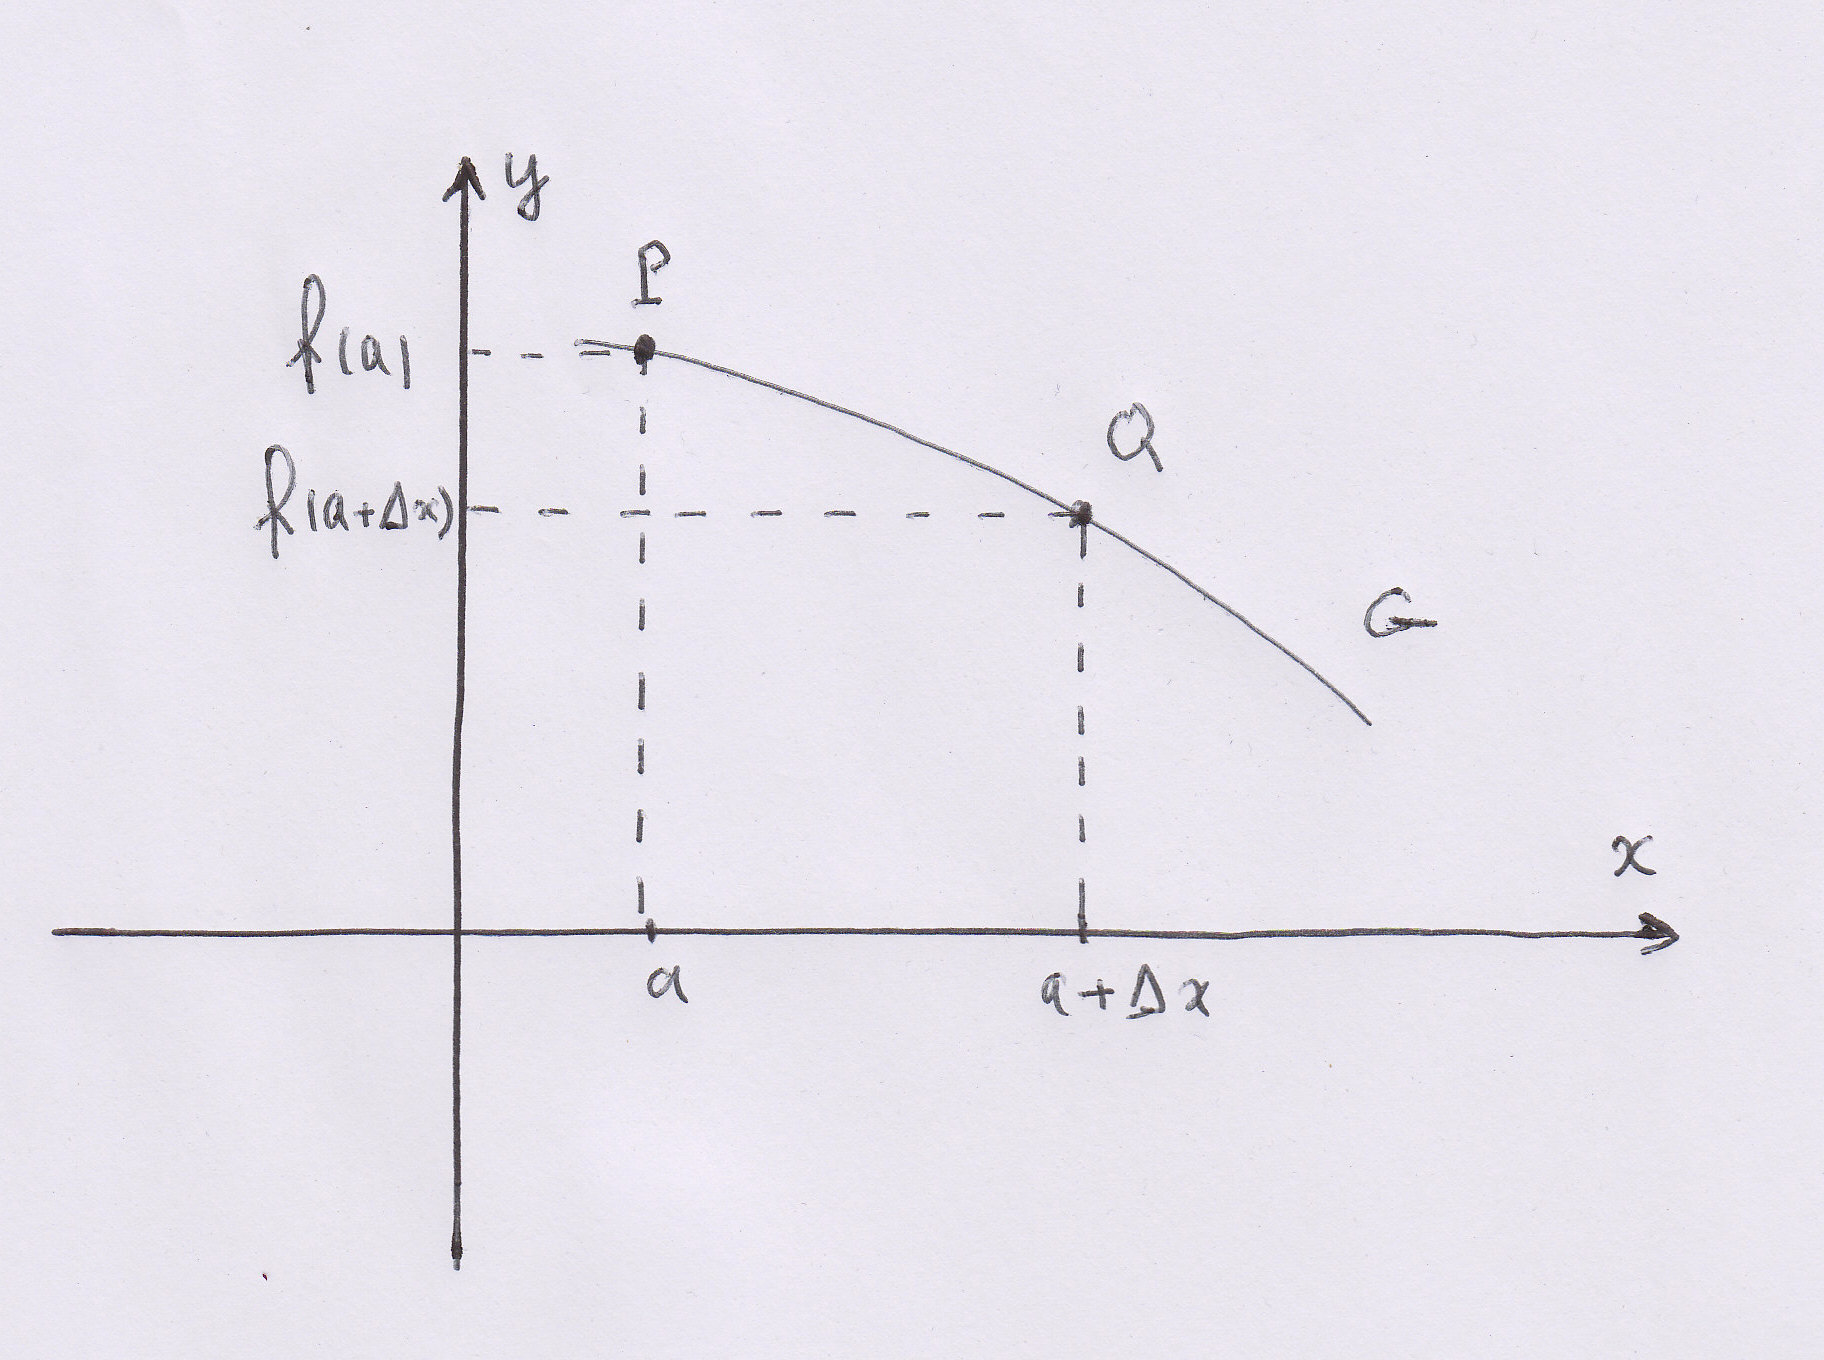
\includegraphics[height=5 cm]{6_afgeleiden_integralen/inputs/dalend.JPG}
%	\end{center}
%\end{figure}

In zulk geval heet de functie $f$ dalend in $a$.\vspace{5mm}

Op dezelfde manier bekom je dat als $Df(a)>0$ dan is de functie stijgend in $a$.
Je bekomt de volgende verbanden tussen $Df$ en het verloop van $f$.

\begin{eigenschap}
Als de eerste afgeleide $f'(x)>0$  is in een interval, dan zal de functie in dat interval \textbf{stijgen}.

Als de eerste afgeleide $f'(x)<0$ is in een interval, dan zal de functie in dat interval \textbf{dalen}.

De functie zal een \textbf{relatief of lokaal extremum (maximum of minimum)} bereiken waar de kromme overgaat van een stijgende naar een dalende functie of omgekeerd. Dit gebeurt wanneer de eerste afgeleide van teken verandert.

Een functie $f(x)$  heeft in het punt $(x_0,y_0)$ een extremum (relatief minimum of relatief maximum) als in dat punt aan volgende voorwaarden voldaan zijn:
$f'(x_0)=0$
en $f''(x_0)\ne 0$
Voor $f''(x_0)> 0$ is het extremum een lokaal minimum.

Voor $f''(x_0)< 0$ is het extremum een lokaal maximum.
\end{eigenschap}

\begin{voorbeeld}
	\begin{eqnarray*}
	f(x) & =& x^3-3x^2 \\
	f(x) & =& 3x^2-6x \\
	f''(x) & =& '6x-6 
	\end{eqnarray*}

\gewonefiguur{width=.5\linewidth}{6_afgeleiden_integralen/inputs/1_9_fig2}
%
%	\begin{figure}[h]
%	\centering
%	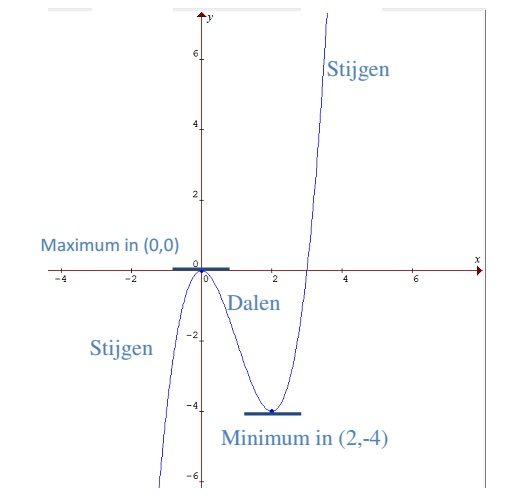
\includegraphics[width=.5\linewidth]{6_afgeleiden_integralen/inputs/verloop_vb2}
%	\caption{Voorbeeld verloop van een functie}
%	\label{fig:verloopvb2}
%\end{figure}


	Voor welke waarden van $x$ is de afgeleide gelijk aan 0? Stel dat $f'(x)=0$, dus
	\begin{equation*}
	3x^2-6x=0,
	\end{equation*}
	maar aangezien $3x^2-6x=3x(x-2)$ moet dan gelden dat
	\begin{equation*}
	3x =0 \text{ of } x-2=0
	\end{equation*}
	dus
	\begin{equation*}
	x=0 \text{ of } x=2
	\end{equation*}
	zodat meteen volgt dat enkel $f'(0)=0$ en $f'(2)=0$.
	
	Om de $y$-co\"ordinaat van de bijhorende punten te vinden, berekenen we de functiewaarden van $f$ in $0$ en $2$. We vinden
	\begin{eqnarray*}
		f(0)&=&(0)^3-3.(0)^2= 0 \\
		f(2)&=&(2)^3-3.(2)^2= 8-12=-4 \\
	\end{eqnarray*}
	De functie bezit in die punten $(0,0)$ en $(2,-4)$ dus een horizontale raaklijn. Zijn de punten ook extrema? 
	Aangezien $f''(0)=-6<0$ is het punt $(0,0)$ een lokaal maximum. Verder is $f''(2)=6>0$ en dus is $(2,.4)$ een lokaal minimum.
	
	Aangezien de eerste afgeleide een tweedegraadsfunctie is, zullen we het tekenverloop van de tweedegraadsfunctie toepassen.
	
	\begin{center}
		\begin{tabular}{c|ccccc}
			$x$ & & 0 & & 2 & \\
			\hline 
			$f'(x)$ & + & 0 & - & 0 & + \\
			\hline
			$f(x)$ & $\uparrow$  & $\frac{0}{\text{max}}$ & $\downarrow$ & $\frac{-4}{\text{min}}$ & $\uparrow$
		\end{tabular}
	\end{center}


\end{voorbeeld}

\subsection{Test afgeleiden}
%TODO





